\section{Remediation of demo}

In the demostration of the simulator, a defect was found which ultimately prevented one of the tests to pass because of runtime error.
The test in question was "recursive.bin". The problem was with the decoding of the J immediate format.
The problem's root cause was a misinterpretation of the specification. 
On page 17 of the official RISC-V RS32I specification, it was misinterpreted that instr[20] should be extended, in a similar manner to instr[31].
The following illustration visualize how the misinterpretation was made with a view in a hasty manner.
\begin{center}
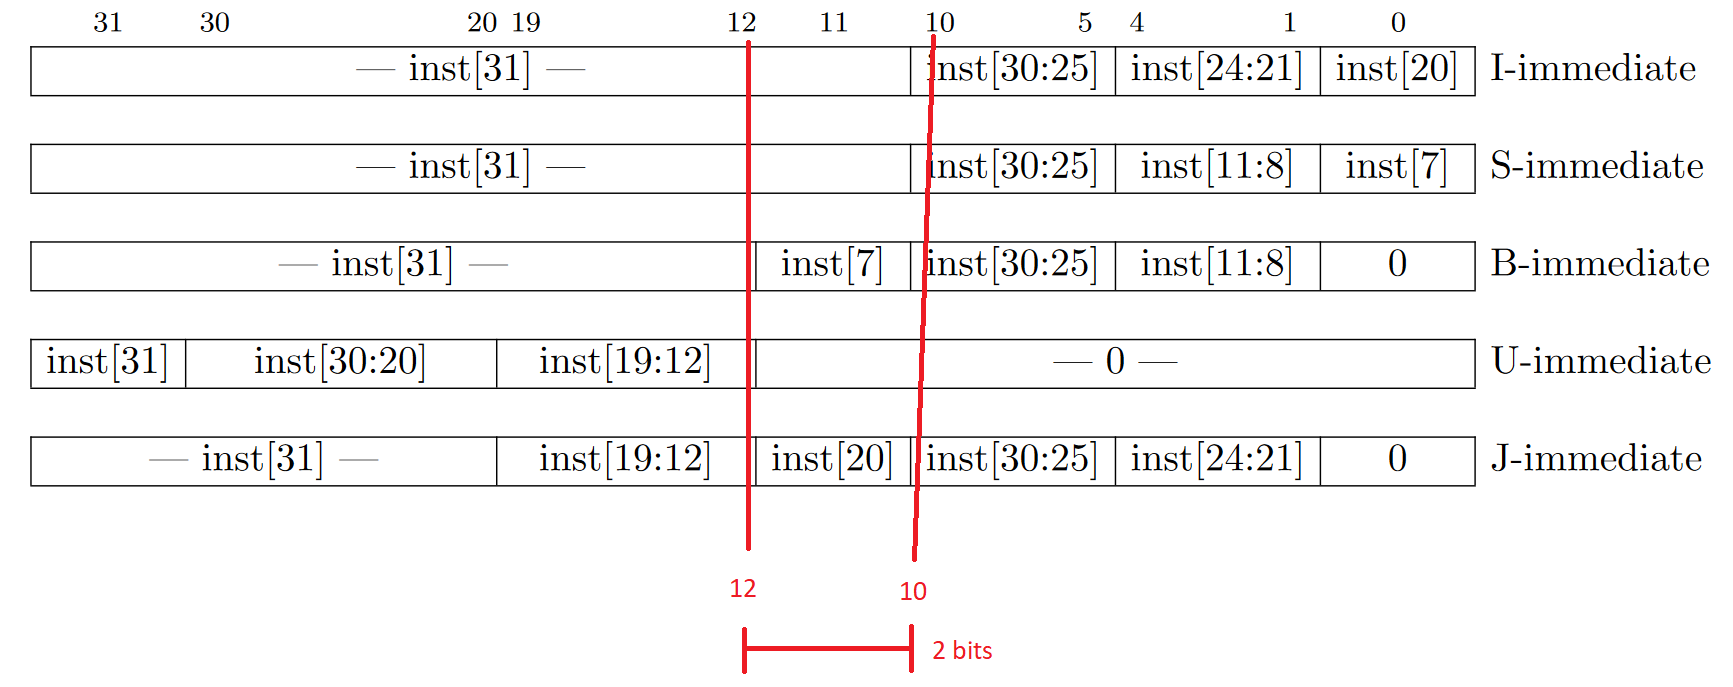
\includegraphics[width=1\textwidth]{images/immediate.png}
\end{center}



This misinterpretation caused an incorrect decoding implementation, which caused incorrect behavior from instructions using the J format (in this case only jal).
After becomming aware of the misunderstanding, the J immediate decoding was then fixed resulting in a similar behavior to that of ripes running the same binary.

\begin{wrapfigure}[19]{r}{0.65\textwidth}
    \centering
    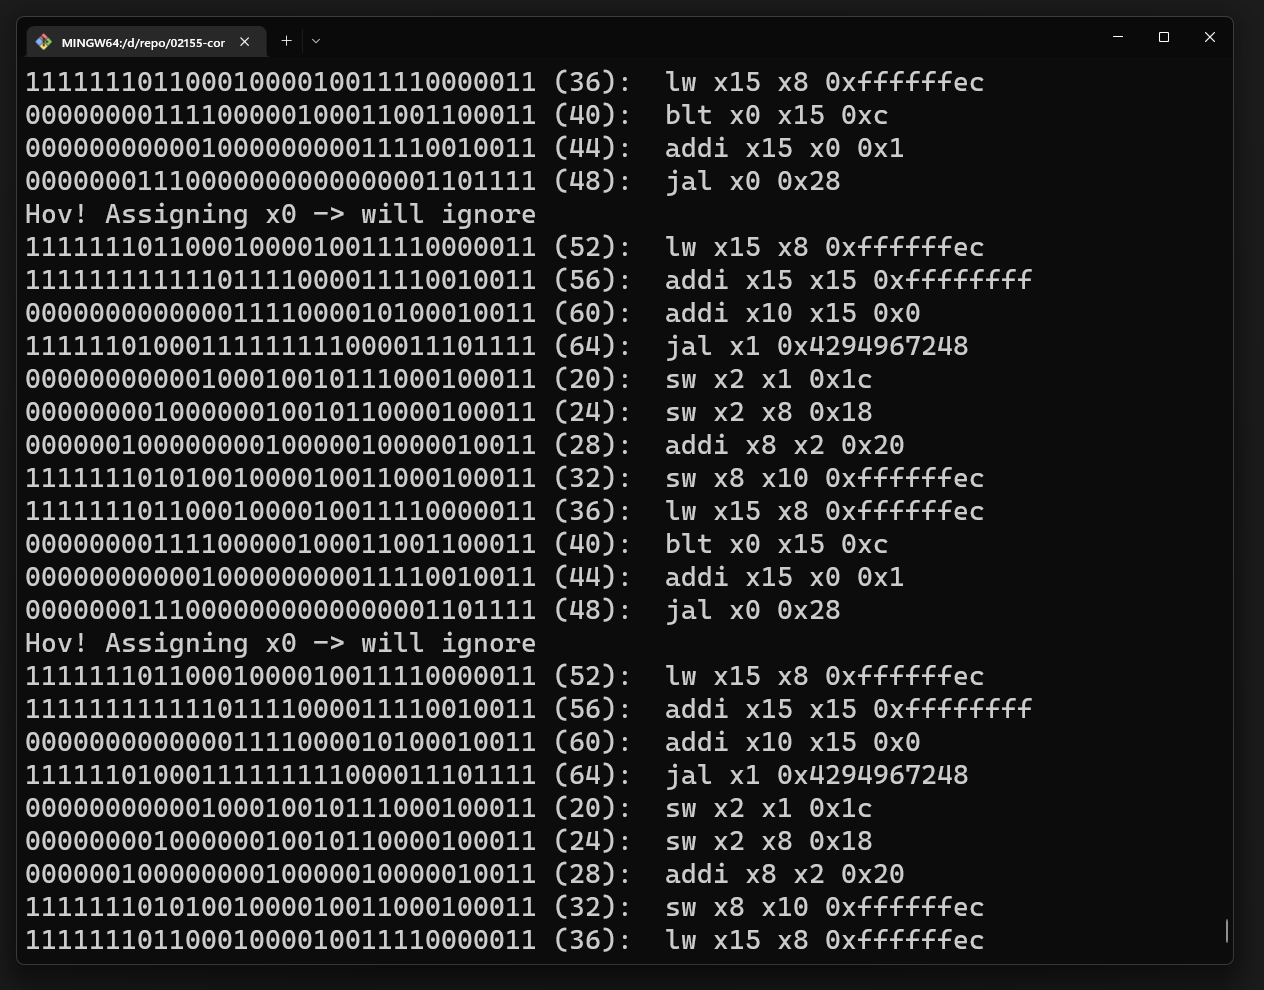
\includegraphics[width=0.65\textwidth]{images/loop.png}
\end{wrapfigure}

\hspace{2em}

To be extra sure, "recursive.bin" was manually downloaded from the assignment repository.
Simulating "recursive.bin" will similarly to ripes, get stuck in an endless loop. 
The screenshot prints debug information of the instructions being executed in the endless loop.
The screenshot captures 2 iterations of the loop.

Looking at the code in recursive.c, it should return with exit code 101. 
Hence, recompiling recursive.c instead of using binary file from assignment repository and running it succesfully terminates, but not with same results as from the assignment repository.
I suspect that the compilation of the recursive.c has been done with different methods that has descrepencies.